\documentclass[a4paper,10pt,twoside]{report}
\usepackage[a4paper]{geometry}
\usepackage{listings}
\usepackage[latin9]{inputenc} % ISO 8859-1
\usepackage[ngerman]{babel}
\usepackage{color}
\usepackage[pdftex]{graphicx}
\usepackage{fancyhdr}
\usepackage{amsmath,amssymb,amsfonts,textcomp}
\usepackage{hyperref}
\usepackage[compact]{titlesec} % Kapitel�berschriften
\usepackage[T1]{fontenc}
\usepackage{xspace}



% Dateipfade
\graphicspath{{pictures/}}

% Eigene Farben
\definecolor{lightgray}{rgb}{0.95,0.95,0.95}
\definecolor{codegray}{rgb}{0.8,0.8,0.8}
\definecolor{darkgray}{rgb}{0.18,0.18,0.18}
\definecolor{mygreen}{rgb}{0.133,0.545,0.133}
\definecolor{mypurple}{rgb}{0.627,0.126,0.941}

% PDF Informationen
\title{Beispieldokumentation zum Projektpraktikum}
\author{Hier bitte Autor eintragen}

% Seitengestaltung
\setlength\textheight{25.0cm}
\setlength\topmargin{-1.3cm}
\setlength\textwidth{1.1\textwidth}
% ohne Heftkante
\setlength\oddsidemargin{0pt}
\setlength\evensidemargin{0pt}
% mit Heftkante
%\setlength\oddsidemargin{+10pt}
%\setlength\evensidemargin{-10pt}
\setlength{\headheight}{13pt}

% Kopf- und Fußzeilen
\pagestyle{fancy}
\fancypagestyle{plain}{\thispagestyle{fancy}}

\fancyhead{}
%\fancyheadoffset[LE,RO]{0pt}
\fancyhead[LO,RE]{\rightmark} % aktuelle Section
\fancyhead[RO,LE]{
\includegraphics[viewport=0 7.5 168 24,scale=0.5]{header}} % Logo here

\fancyfoot{}
%\fancyfootoffset[LE,RO]{0pt}
\fancyfoot[LO,RE]{\leftmark} % aktuelle Chapter
\fancyfoot[LE]{\thepage\hspace{3em}Dokumentation zum IT-Projektpraktikum} %Seitenzahl links
\fancyfoot[RO]{Dokumentation zum IT-Projektpraktikum\hspace{3em}\thepage} %Seitenzahl recht

% Titel Linie
\newcommand{\bigrule}{\titlerule[0.5mm]}

% Titel Format
\titleformat{\chapter}[display]
{\bfseries\Huge}
{%
 \vskip-2em
 \titlerule
 \filright
 \Large\chaptertitlename\
 \Large\thechapter
}
{0mm}
{\filright}
[\bigrule]

% Definitionen f�r Listing
\lstset{ %
language=C++,                % choose the language of the code
numbers=left,                   % where to put the line-numbers
%numberstyle=\footnotesize,      % the size of the fonts that are used for the line-numbers
stepnumber=1,                   % the step between two line-numbers. If it's 1 each line will be numbered
numbersep=5pt,                  % how far the line-numbers are from the code
backgroundcolor=\color{white},  % choose the background color. You must add \usepackage{color}
showspaces=false,               % show spaces adding particular underscores
showstringspaces=false,         % underline spaces within strings
%showtabs=false,                 % show tabs within strings adding particular underscores
frame=single,                   % adds a frame around the code
tabsize=2,                      % sets default tabsize to 2 spaces
captionpos=t,                   % sets the caption-position to bottom
breaklines=true,                % sets automatic line breaking
xleftmargin=3.5pt,
xrightmargin=3.5pt,
breakatwhitespace=false,        % sets if automatic breaks should only happen at whitespace
extendedchars=true,captionpos=t , prebreak=\mbox{$\hookleftarrow$}, belowcaptionskip=0.5em,postbreak={},
basicstyle=\ttfamily,       % the size of the fonts that are used for the code
keywordstyle=\color{blue}\bfseries\sffamily,
commentstyle=\color{mygreen}\slshape,
stringstyle=\color{mypurple},
}

\setlength{\parindent}{0pt} % Texteinzug bei neuem Absatz

% Zähler für Ausgabe
\newcounter{ausgabe}[chapter]
\renewcommand\theausgabe{\thechapter.\arabic{ausgabe}}

% Programmausgabe, grau hinterlegen
\newcommand{\ausg}[2]{
	\stepcounter{ausgabe}

	\vspace{2mm}
	\begin{minipage}{\textwidth}
	  \colorbox{codegray}{
			\begin{minipage}{0.97\textwidth}
				\textbf{\texttt{#2}}
			\end{minipage}
		}
		\begin{center}
			Ausgabe \theausgabe: #1
		\end{center}
	\end{minipage}
}

% Schreibt 'Code::Blocks'
\newcommand{\cb}{\mbox{Code::Blocks}\xspace}

% Schreibt 'Visual Studio'
\newcommand{\vs}{\mbox{Visual Studio}\xspace}

% TODO - Command
\newcommand{\TODO}[1]{{\color{red}TODO!! #1}}

% code - Command
\newcommand{\code}[1]{
\section{#1}
\lstinputlisting{../#1}
\newpage
}

% Leerseite ohne Seitennummer, nächste Seite rechts
\newcommand{\blankpage}{
 \clearpage{\pagestyle{empty}\cleardoublepage}
}



\begin{document}
%----------------------------
\begin{titlepage}
	\begin{flushleft}
		\begin{picture}(0,0)
			\put(0,-2){
\includegraphics[height=4em]{KIT_Logo.pdf}}
		\end{picture}
			\put(140,14){\Large Karlsruher Institut f�r Technologie}
			\put(120,0){\large Institut f�r Technik der Informationsverarbeitung}
		\begin{picture}(0,0)
			\put(410,-2){
\includegraphics[height=4em]{itiv}}
		\end{picture}
	\end{flushleft}

	\begin{center}
		\vspace{7cm}
		\addvspace{1.0cm}
		\Huge {Dokumentation zum Projektpraktikum Informationstechnik}\\
	\end{center}
	\vspace{4.0cm}
	\Large

	\begin{flushleft}
	\begin{tabular}{ll}
		Gruppe:& 064\\
		Gruppenmitglieder:& Benedikt Braunger, Cornelius Richt,\\ & Fabian Schackmar, Lukas Mohrbacher\\
		Tutor:& Florian Brauchle\\
		Abgabetermin:& 18.01.2013\\
		Semester:& WS2011/2012
	\end{tabular}

	\vfill

	KIT - Universit�t des Landes Baden W�rttemberg und nationales Forschungszentrum in der Helmholtz-Gemeinschaft
	\end{flushleft}
\end{titlepage}
%----------------------------
\tableofcontents
\chapter{Einleitung}
Im folgenden wird die Umsetzung eines Programmes f�r die CoolSoft AG im Rahmen des Informationstechnik-Praktikums f�r den Studiengang Elektro- und Informationstechnik beschrieben.
\\
\\
Es wird als erstes auf die allgemeine Problemstellung eingegangen. Nachfolgend beschreiben wir dann besonderheiten unserer L�sung und Probleme die w�hrend des bearbeiten aufgetreten sind. Schlussendlich ist dann nat�rlich noch der komplette Code abgebidruckt.
\\
\\
In einem umfangreichen Praktikumspaket wurde der genaue Programmaufbau erl�utert, inklusive Klassendiagramm. F�r einzelne Programmteile wie zum Beispiel die Analyse und Tiefensuche wurde Pseudocode vorgegeben. Somit ging es im allgemeinen nur um die Realisation in C++.

\begin{figure}[h]
\centering
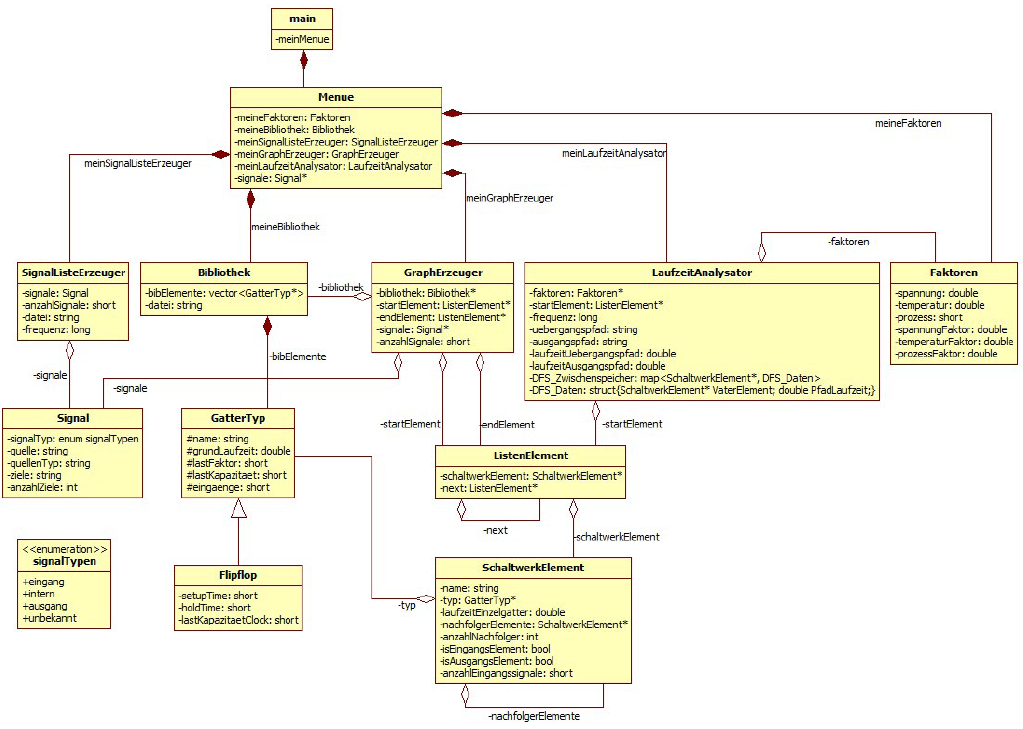
\includegraphics[width=\textwidth]{pictures/schema.png}
\caption{Klassendiagramm}
\end{figure}
\chapter{Aufgabenstellung}
In der gegebenen Aufgabe, soll ein Schaltnetz, welches in Form einer Schaltnetzdatei gegeben ist, analysiert und
auf Fehler untersucht werden. Dann soll die maximal m�gliche Frequenz berechnet werden. Das Programm soll
dabei in der C++ Programmiersprache umgesetzt werden.
Um die gew�nschten Funktionen erm�glichen zu k�nnen, muss zun�chst die gegebene Bibliotheksdatei,
welche spezifische Informationen �ber m�gliche Schaltwerkelemente enth�lt, ausgelesen werden und die
Informationen in eine passende Datenstruktur �berf�hrt werden. Zus�tzlich m�ssen �u�ere Einfl�sse auf
die Laufzeit (Betriebsspannung, Temperatur und Herstellungsprozess) in Faktoren umgerechnet werden.
Anschlie�end kann die eigentliche Schaltnetzdatei, welche die Schaltnetzstruktur in Form von Signalen
mit entsprechenden Quellen und Zielen darstellt, ausgewertet werden. Auch hier m�ssen die Informationen
in einer geeigneten Datenstruktur gespeichert werden. Erst jetzt kann die eigentliche Funktion des
Programms ausgef�hrt werden. Dazu wird mit Hilfe der Signale ein Schaltnetzgraph erstellt, welcher mit
Hilfe des Tiefensuchalgorithmus in einen Tiefenbaum �berf�hrt wird. Damit kann dann die maximale Frequenz
berechnet werden.
Dar�ber hinaus wurde gefordert, das gesamte Programm komfortabel �ber das Windows Command Window
steuern zu k�nnen.

Jedes reale Bauteil weist eine gewisse zeitliche Verz"ogerung zwischen Ein- und Ausgangssignal auf. F"ur den vorliegenden Fall in Abbildung 2.1 bedeutet dies, dass das Ausgangssignal des 1. Flipflops eine gewisse Zeit braucht, bis es im Und-Gatter verarbeitet wurde und am Eingang des 2. Flipflops anliegt.

\begin{figure}[h]
 \centering
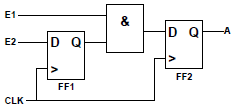
\includegraphics[]{pictures/einfach.png}
\caption{Einfaches Schaltwerk}
\end{figure}

Daraus folgt, dass das zweite Flipflop erst dann getriggert werden darf, wenn das Signal dort sicher
angekommen ist. Es gibt also eine maximale Taktfrequenz mit der die Schaltung betrieben werden darf.
Diese zu finden ist Aufgabe des Programms. Dazu muss das Programm den l"angsten Signalpfad finden
und dessen Laufzeit berechnen. Die Laufzeit h"angt noch von diversen �u�eren Einfl"ussen wie Temperatur
und Spannung ab, die ebenfalls ber"ucksichtigtigt werden sollen.

\begin{figure}[h]
\centering
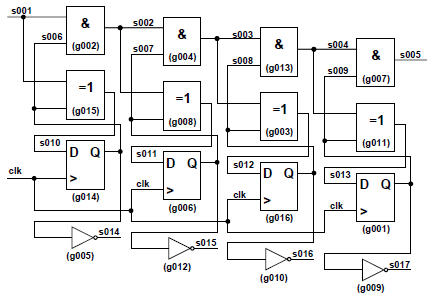
\includegraphics[width=\textwidth]{pictures/rueckwaerts.png}
\caption{R�ckw�rtsz�hler}
\end{figure}

 Dieser R�ckw�rtsz�hler stellt im Projektpraktikum das Beispielschaltwerk dar, welches untersucht werden soll.
\chapter{Umsetzung}

\section{Zeitplanung}
Im ersten Tutorium verschafften wir uns einen groben "Uberblick "uber die Aufgabenstellung und besprachen die Vorgehensweise. Die Umsetzung folgte in den n"achsten Tutorien bis zu den Abschlusstest und der Pr"asentation vor dem Tutor.
Wie an der Git-Grafik zu sehen ist wurde die M�glichkeit Donnerstags an der Uni w�hrend des Tutoriums zu arbeiten intensiv und fast ausschlie�lich genutzt.

\begin{figure}[h]
\centering
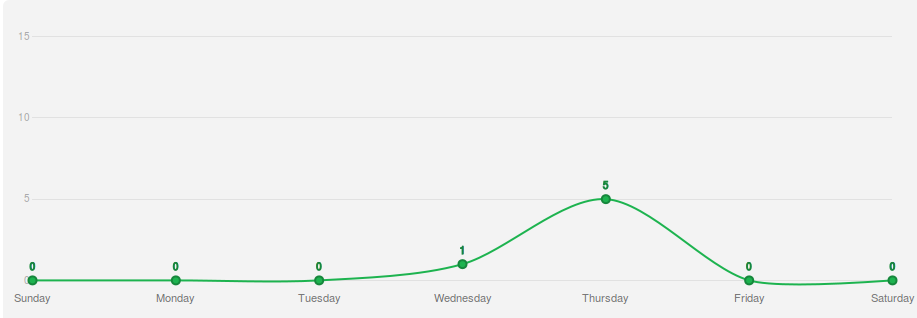
\includegraphics[width=\textwidth]{pictures/git-commits.png}
\caption{Git: Durchschnittliche Commits nach Wochentag}
\end{figure}

\section{Materialien}
\subsection{Programmierumgebung}
Als Programmierumgebung wurde haupts�chliche \textbf{\cb} verwendet da ein Gro�teil der Gruppe Linux nutzt und dort kein Visual Studio l�uft. Kompiliert wurde mit dem gcc, da dieser Compiler unter Linux wie auch Windows mit nahezu dem gleichen Quellcode auskommt. Mehr dazu im Abschnitt Kompatibilit�t.

\subsection{Versionsverwaltung}
Der Austausch des Fortschrittes untereinander wurde mit der Versionsverwaltung \textbf{Git} gemacht. Als Zentrales Repository wurde der kostenlose Service von Github genutzt. Git erm�glicht es mit geringem Aufwand den Quellcode untereinander synchron zu halten und gleichzeitig auch eine History f�r "Anderungen am Quellcode zu haben.

\subsection{Dokumentation}
Zur Dokumentation verwendeten wir \textbf{\TeX} denn dies spielt mit der Versionsverwaltung Git am besten zusammen und es ist keine aufwendige Formatierung des Dokumentes n�tig.


\newpage
\section{Besondere Codeabschnitte}
\subsection{Allgemein}
Bibliothek, Gattertyp, Flipflop, Signale und Listenelement sind prinzipiell nur Umsetzung der Prototypen in der Aufgabenstellung bzw. des Angegeben Pseudocodes. Code-Abschnitte die etwas spezieller sind odder von der Aufgabenstellung abweichen sind in diesem Abschnitt erl�utert.

\subsection{Klasse �u�ere Faktoren (faktoren.h/ *.cpp)}
Diese Klasse beinhaltet Attribute und Methoden, um aus den physikalischen Randbedingungen der Schaltung Faktoren zu errechnen, die in der Laufzeitanalyse sp�ter gebraucht werden. Alle Attribute werden als private angelegt und man kann nur mittels der f�r die 3 Attribute Spannung,  Temperatur und Prozess geschriebenen �ffentlichen get- und set-Methoden darauf zugreifen.  Die 3 Faktorattribute werden in den nach ihnen benannten privaten Methoden (berechneXFaktor(..)) mittels der in ihnen als zweidimensionale Arrays gespeicherten Listen,  die 3 (Prozess: slow, typical, fast), 7 (Spannung: 1,08 - 1,32V) oder  15 (Temperatur: -25 ? 125�C) Werten einen Faktor zuweisen, berechnet. 

Diese schlie�en zuerst h�here bzw. niedrigere  Eingaben als die zugelassenen aus ? durch Ausgabe einer Fehlermeldung ? und rufen dann allesamt die private Methode "berechneFaktor (?)" auf,  der sie den Array, die Array-Zeilenanzahl und den Wert der Randbedingung �bergeben. Die Methode durchsucht das �bergebene Array  vom kleinsten Eintrag an nach dem �bergebenen Wert, wobei  sie f�r jeden Listeneintrag (im Array), den der Wert �berbietet, eine untere Schranke und dessen direkter Nachfolger in der Liste als obere Schranke festlegt.

 Existiert der gesuchte Wert in der Liste wird sofort der diesem zugeordnete Faktor zur�ckgegeben, wenn nicht, wird die private Methode "interpolation(..)" mit dem Wert, der unteren und oberen Schranke, sowie deren zugeordnete Faktoren als Parametern aufgerufen. Diese berechnet aus den 4 Schrankenwerten (2 Punkte) eine Geradengleichung (m*x +n) und kann somit dem Wert den gesuchten Faktor zur�ckgeben. 

Des Weiteren sind ist noch eine �ffentliche Displayausgabefunktion (ausgabeFaktoren() ) f�r die errechneten Faktoren implementiert und �ffentlich get-Methode, die alle 3 berechneten Faktoren per Referenz�bergabe zur�ckgibt( getFaktoren(?)). Der Konstruktor initialisiert s�mtliche Attribute mit 0.

Zum Testen wurde eine eigene Main-Datei geschrieben (FaktorenTestMain.cpp), die zuerst eine Klasse vom Typ �u�ere Faktoren anlegt. Dann werden via Konsoleneingabe die 3 �u�eren Randbedingungen Spannung, Temp. und Prozess �bergeben, �ber die set-Methoden gesetzt und zur Kontrolle die Faktoren (alle zu diesem Zeitpunkt 0) und eingegebenen Werte ausgegeben , dann berechnet und im Anschluss werden die Faktoren ? nun mit den richtigen Werten - noch einmal ausgegeben. F�r jede Bedingung wurden ung�ltige Werte eingesetzt, die alle abgefangen wurden.

\lstinputlisting[caption={FaktorenTestMain.cpp}]{../FaktorenTestMain.cpp}

\subsection{SignalListeErzeuger}
Diese Klasse liest die Signaldatei Zeilenweise ein und aufgrund unterschiedlicher Zeilenanf�nge werden diese dann interpretiert, im Gegensatz zur Vorgabe wurden die Signale nicht in einem dynamischen Array gespeichert sondern in einem Vektor da dieser einiges flexibler ist als ein Array.
Die Ergebnisse dieser Funktion wurden vor der Fertigstellung des Programmes mit der Datei Signal\_test\_main.cpp getestet.

\lstinputlisting[caption={Signal\_test\_main.cpp}]{../SIGNAL_TEST_MAIN.cpp}

\subsection{Bibliothek}
Stellvertretend f�r alle Men�punkte ist hier das Bibliotheksmen� abgebildet, der Ablauf ist immer gleich.

Erst wird mit der Funktion menueKopf der Header ausgegeben, dann die Men�punkte und dann wird eine Zahl f�r den jeweiligen Men�punkt abgefragt. Das ganze kommt noch in eine Endlosschleife die mit einem anderen Men�punkt abgebrochen werden kann und fertig ist das Men�.

\begin{figure}[h]
\caption{Menue::bibliothekMenue()}
\begin{lstlisting}
void Menue::bibliothekMenue()
{
    /**
     Im Untermen� der Bibliothek soll der Pfad zur Bibliotheksdatei ge�ndert werden k�nnen und man
    soll sich zur Kontrolle auch die Datei im Men� anzeigen lassen k�nnen. Auch die Klasse Bibliothek
    stellt dazu eine Ausgabemethode bereit.
    */

    string pf;
    while(input != "3") {
        menueKopf();
        cout << "Untermenue Bibliothek" <<endl;
        cout << "(1) Pfad zur Bibliotheksdatei: " << meineBibliothek.getPfad() <<endl;
        cout << "(2) Ausgabe der Bibliotheksdatei" << endl;
        cout << "(3) Hauptmenue" << endl<< endl;
        cout << "Waehle einen Menuepunkt und bestaetige mit Enter: ";

        getline(cin, input);
        switch (atoi(input.c_str())) {
        case 1:
            cout <<"Pfad eingeben: ";
            cin >> pf;
            if(!meineBibliothek.pfadEinlesen(pf)){
                cout << "Fehler beim einlesen!" << endl;
                cin.get();
            } else {
                meineBibliothek.dateiAuswerten();
                meinGraphErzeuger.setBibliothek(&meineBibliothek);
            }
            break;
        case 2:
            meineBibliothek.dateiAusgabe();
            cin.get();
            break;
        }
    }
    input.clear();
}
\end{lstlisting}
\end{figure}



\begin{figure}[h]
\caption{Menue::menueKopf()}
\begin{lstlisting}
void Menue::menueKopf()
{
    /**
    Gibt den Kopf der Men�s aus. Dieser bleibt in Hauptmen� und allen Untermen�s gleich.
    */
    clear_screen();
    cout << " ****************************************** \n *     IT-Projektpraktikum WS2012/2013    * \n *                                        * \n * Laufzeitanalyse synchroner Schaltwerke * \n ******************************************" << endl << endl; //Ausgabe des "Headers"
}
\end{lstlisting}
\end{figure}

\subsection{Plattform unabh�ngigkeit}
Da wir gemischt unter Windows und Linux programmiert haben wollten wir das Programm nat�rlich nicht nur unter beiden Betriebssystemen kompilieren sondern auch nutzen k�nnen. Dabei traten zwei Probleme auf.
\subsubsection{Konsole l�schen}
F�r den clear Befehl benutzen die beiden Betriebssysteme unterschiedliche Funktionen. Diese sind jedoch in zwei Bibliotheken zu finden und somit musste nur die jeweilige Funktion einfach aufgerufen werden. Um herauszufinden unter welchem System man gerade kompiliert stellt der compiler eine FLAG zur verf�gung die man dan ganz einfach auslesen kann. Dieses auslesen passiert in der Funktion clear\_screen().
\lstinputlisting[caption={cross-compatibility.cpp}]{../cross-compatibility.cpp}

\subsubsection{Zeilenendung}
Windows und Linux definieren die Zeilenendung unterschiedlich, und zwar wird gibt es zwei Funktionen, zum einen \textbackslash n f�r newline und \textbackslash r f�r carriage returns was denn Zeiger an den Anfang der Zeile verschiebt. Windows nutzt nun \textbackslash n \textbackslash r hintereinander um ein Zeilenende zu formulieren, und unter Linux reicht \textbackslash r. Nun f�hrt diese unterschiedliche Konvention dazu das man unter Windows ein Zeichen zu wenig subtrahiert wenn man die funktion String.substr() nutzen m�chte. Daher der define Linuxzusatz (was aber eigentlich ein Windowszusatz ist).

\subsubsection{Debug ausgabe}
Um die Ausgabe von debug Nachrichten variabel je nach Debug oder Release zu erm�glichen gibt es die zwei defines, debug\_msg() und debug\_pause(). Hier wird aufgrund des Defines DEBUG entschieden ob die Nachricht jetzt ausgegeben werrden soll oder nicht.
\lstinputlisting[caption={cross-compatibility.h}]{../cross-compatibility.h}

\newpage
\section{Abschlusstest}
Nach der Fertigstellung des Programms testeten wir es mit verschiedenen Fehlerhaften Dateien um eventuelle Kurzschl"uesse oder Zyklen im Schaltnetz zu finden und die richtige Fehlermeldung ausgeben zu k�nnen. Zudem verglichen wir die ausgebenen Ergebnisse und pr"uften sie auf Richtigkeit

Wir testeten folgende Dateien, welche alle zur richtigen Fehlerausgabe f"urten 
	\begin{itemize}
	\item test Kurzschluss.txt 
	\item test UnbenutztesSignal.txt 
	\item test zyklus.txt
	\item test OffenerEingang.txt  
	\item test Zyklus1.txt           
	\item Test Schaltnetze.pdf     
	\item test Zyklus2.txt           

	\end{itemize}
\chapter{Fazit}
\appendix
\chapter{Quelltext}
\code{main.cpp}
\code{Menue.h}
\code{Menue.cpp}
\code{Faktoren.h}
\code{Faktoren.cpp}
\code{Bibliothek.h}
\code{Bibliothek.cpp}
\code{GatterTyp.h}
\code{GatterTyp.cpp}
\code{Flipflop.h}
\code{Flipflop.cpp}
\code{SignalListeErzeuger.h}
\code{SignalListeErzeuger.cpp}
\code{signals.h}
\code{signals.cpp}
\code{SchaltwerkElement.h}
\code{SchaltwerkElement.cpp}
\code{ListenElement.h}
\code{ListenElement.cpp}
\code{GraphErzeuger.h}
\code{GraphErzeuger.cpp}
\code{LaufzeitAnalysator.h}
\code{LaufzeitAnalysator.cpp}
\code{cross-compatibility.h}
\code{cross-compatibility.cpp}

\end{document}
